
\begin{figure}
\begin{subfigure}[b]{0.33\textwidth}
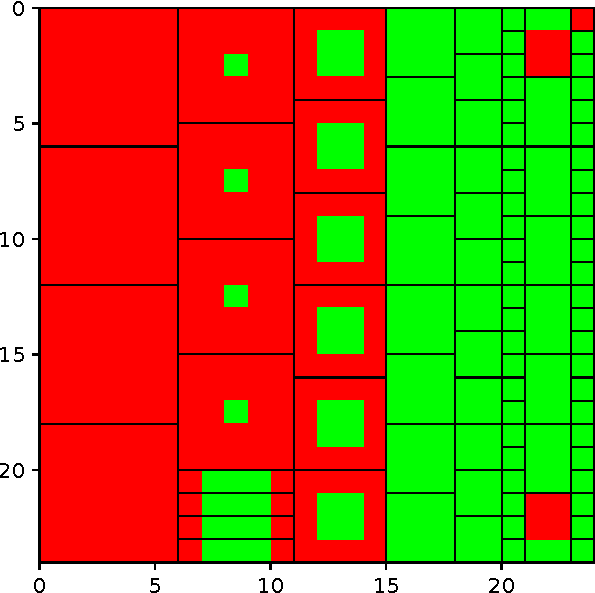
\includegraphics[width=\textwidth]{img/Charm-correctness}
\caption{
Charm++
}
\label{fig:charm_correctness}
\end{subfigure}%
\begin{subfigure}[b]{0.33\textwidth}
  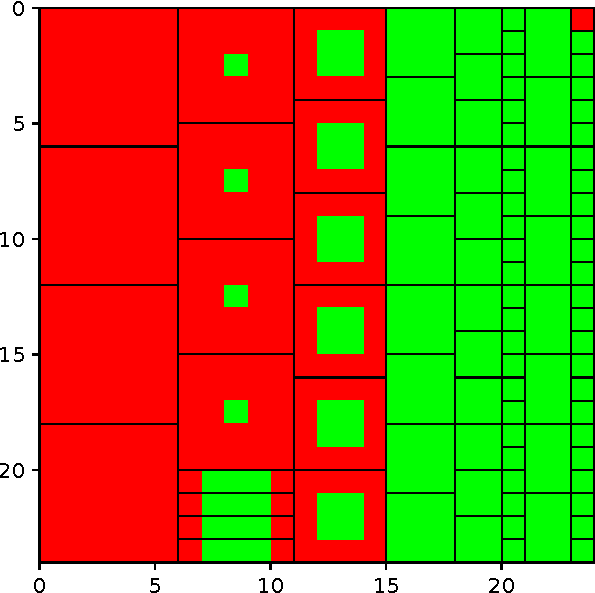
\includegraphics[width=\textwidth]{img/MPI-n1-correctness}
\caption{
MPI $n=1$
}
\label{fig:mpi_n1_correctness}
\end{subfigure}%
\begin{subfigure}[b]{0.33\textwidth}
  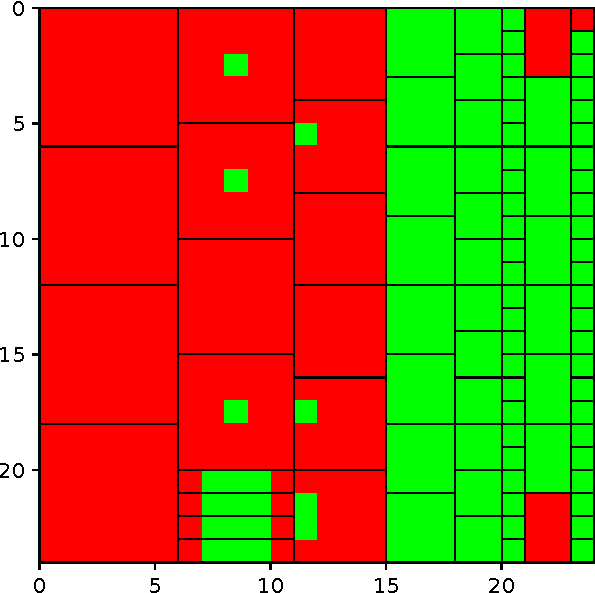
\includegraphics[width=\textwidth]{img/MPI-n4-correctness}
\caption{
MPI $n=4$
}
\label{fig:mpi_n4_correctness}
\end{subfigure}
\caption{
Final resource accumulations as verification of implementation correctness for Charm++ implementation (\subref{fig:charm_correctness}), MPI with $n=1$ (\subref{fig:mpi_n1_correctness}), and MPI with $n=4$ (\subref{fig:mpi_n4_correctness}).
Black lines indicate divisions between same-channel groups.
Red coloring indicates negative resource accumulation at a tile and green coloring indicates positive resource accumulation at a tile.
Note that the single upper-right hand tile is part of a contiguous same-channel group with the large upper-left same-channel group via toroidal wraparound and that the top and bottom $3 \times 2$ same-channel groups in columns 22 and 23 are a contiguous same-channel group via toroidal wraparound.
}
\label{fig:correctness}
\end{figure}
